% Бүлэг 4

\chapter{Системийн хэрэгжүүлэлт ба туршилт}
\label{Chapter4}

\section{Хэрэгжүүлэлтийн зорилго ба хамрах хүрээ}

\paragraph{}
Гуравдугаар бүлэгт хувийн үүлэн хадгалалтын системийн ерөнхий архитектур, үндсэн сервер, дамжуулагч сервер, өгөгдлийн бүтэц болон хэрэглэгчийн интерфейсийн зохиомжийг тодорхойлсон. Энэ бүлэгт тухайн зохиомжийг бодит систем болгон хэрэгжүүлсэн байдал, ашигласан нэвтрүүлэлтийн орчин, системийн холболтын ажиллагаа болон туршилтын үр дүнг авч үзнэ.

\paragraph{}
Хэрэгжүүлэлтийн хүрээнд үндсэн серверийн аппликейшнийг хэрэглэгчийн өөрийн эзэмшлийн Raspberry Pi төхөөрөмж дээр ажиллуулж, алсын хандалтад зориулсан дамжуулагч серверийг Hetzner VPS орчинд байршуулсан. Мөн худалдан авсан домэйн нэрийг VPS-ийн public IP хаягтай холбож, клиент талаас тогтвортой хаягаар системд хандах боломж бүрдүүлсэн. Мобайл хэрэглээний хувьд iOS аппликейшнийг Xcode-ийн development build хэлбэрээр iPhone төхөөрөмж дээр суулган туршсан.

\paragraph{}
Энэ бүлгийн гол зорилго нь боловсруулсан систем зөвхөн онолын зохиомжийн түвшинд бус, бодит төхөөрөмж болон бодит сүлжээний орчинд ажиллах боломжтойг харуулахад оршино. Иймээс нэвтрүүлэлтийн орчин, дотоод болон гадаад сүлжээний холболтын урсгал, хөгжүүлсэн интерфейсүүд, функциональ болон холболтын туршилтуудыг дараах хэсгүүдэд тайлбарлана.

\section{Бодит нэвтрүүлэлтийн орчин}

\paragraph{}
Бодит нэвтрүүлэлтийн орчины хувьд Raspberry Pi 5 болон Hetzner Virtual Public Server худалдан авч программуудыг ажиллуулсан. Хөгжүүлэхээр авсан Raspberry Pi 5 нь 8GB ram-тай хувилбар байсан. Мөн аюулгүй найдвартай ажиллуулахын тулд нэмэлт Active Cooler авч холбосон. Үнийн мэдээллийн хувьд Raspberry PI 5ийг 550,000 төгрөгөөр авсан бол Hetzner-ийн VPS-ийг сарын \$10-оор түрээслэсэн. Үзүүлэлтийн хувьд 2GB RAM, 80GB SSD, 2 core cpu-тэй байгаа. Мөн хөгжүүлэсэн гар утасны application-аа өөрийн гар утас болох iphone 12 mini дээр ажиллуулж туршсан. 

Дараах зураг \ref{fig:working-pi-image}-т ашиглаж буй Raspberry Pi 5-ийн зургийг оруулав. Зурагт харагдаж байгаа pi 5 нь цэнэглэгчтэй холбогдсон бөгөөд 16GB-ийн USB flash drive-тай холбогдсон байгаа юм. Тухайн USB flash drive-ийг энэхүү туршилтынхаа хүрээнд хувийн үүлэн хадгалалтынхаа багтаамжаар ашиглаж байна. Тухайн харагдаж буй хөргүүрийн сэнс нь ачаалал ихэсхэд буюу дотоод температур 50 градус целсээс дээш гарсан тохиолдолд ажиллаж эхэлдэг.

\begin{figure}[H]
    \centering
    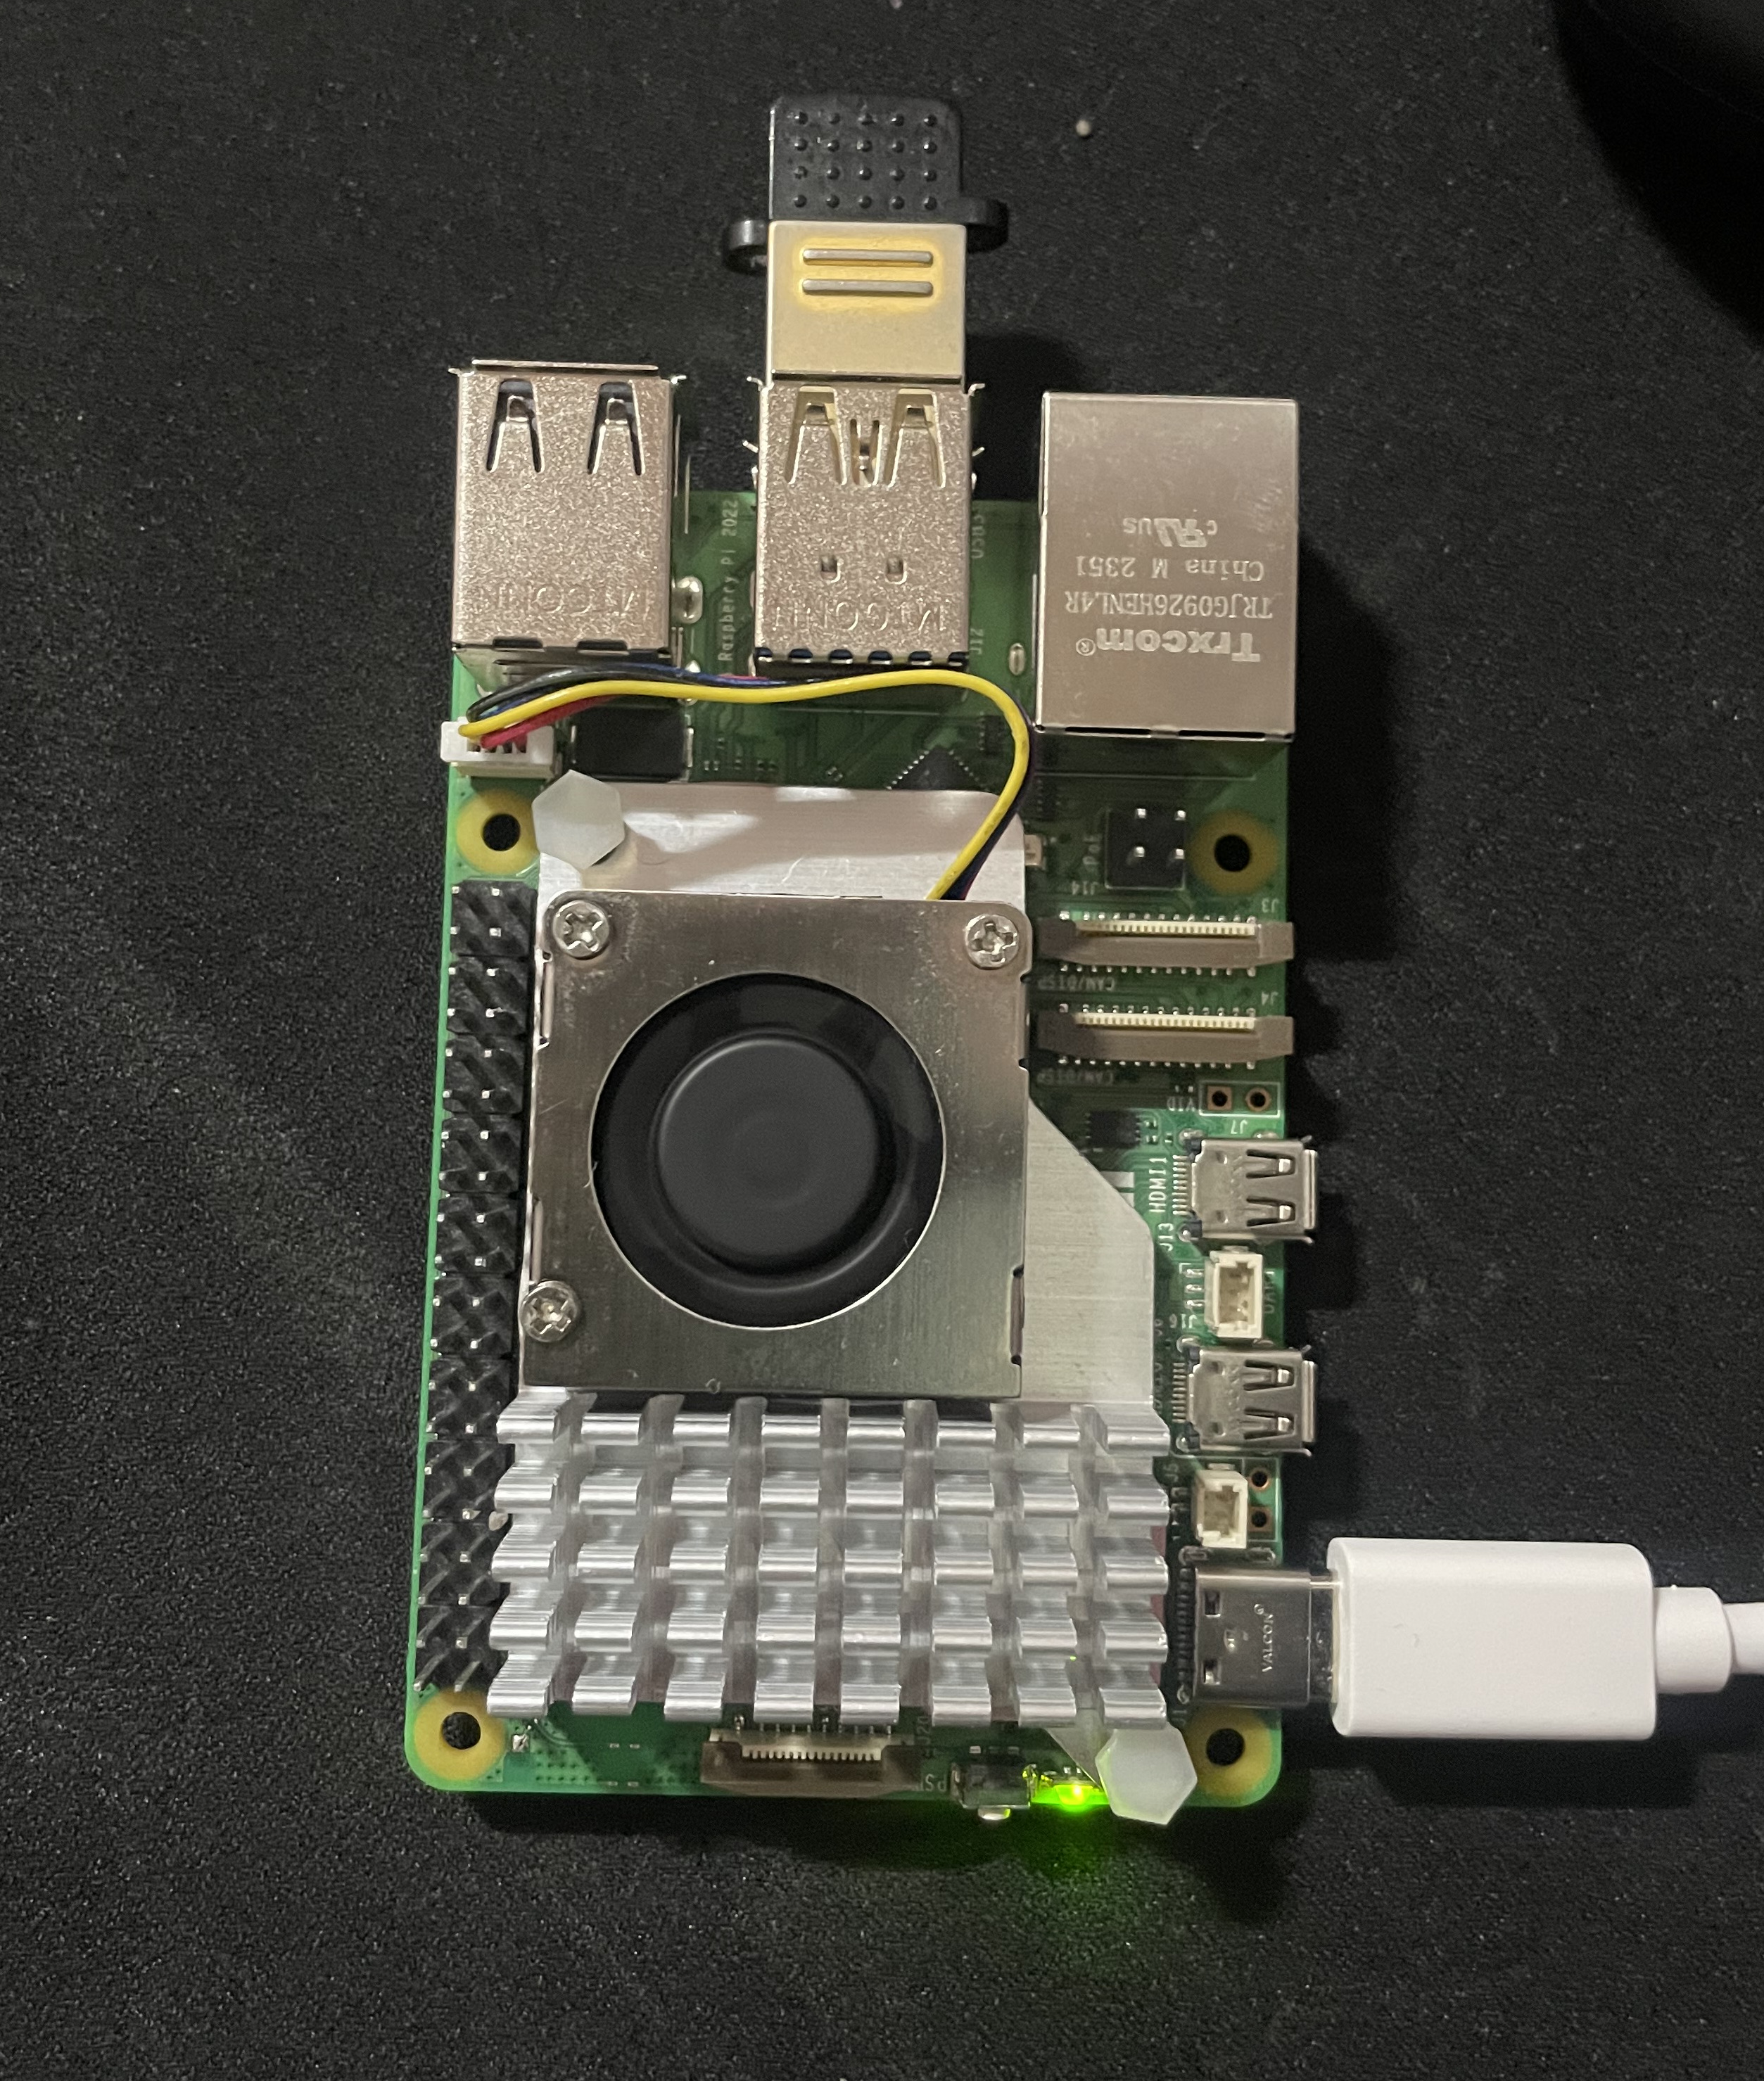
\includegraphics[width=0.55\textwidth]{Figures/chapter4/working-pi-image.jpeg}
    \caption{Ажиллаж буй Raspberry Pi 5}
    \label{fig:working-pi-image}
\end{figure}


Дараах зураг \ref{fig:ssh-pi-main-server-user-service}-т үндсэн үүлэн хадгалалтын сервер аппын хэрэглэгчийн сервис байдлаар ажиллаж байгаа статусыг үзүүлэв. Үүний зэрэгцээ postgre бааз нь docker container ашиглан ажиллаж байгаа.

\begin{figure}[H]
    \centering
    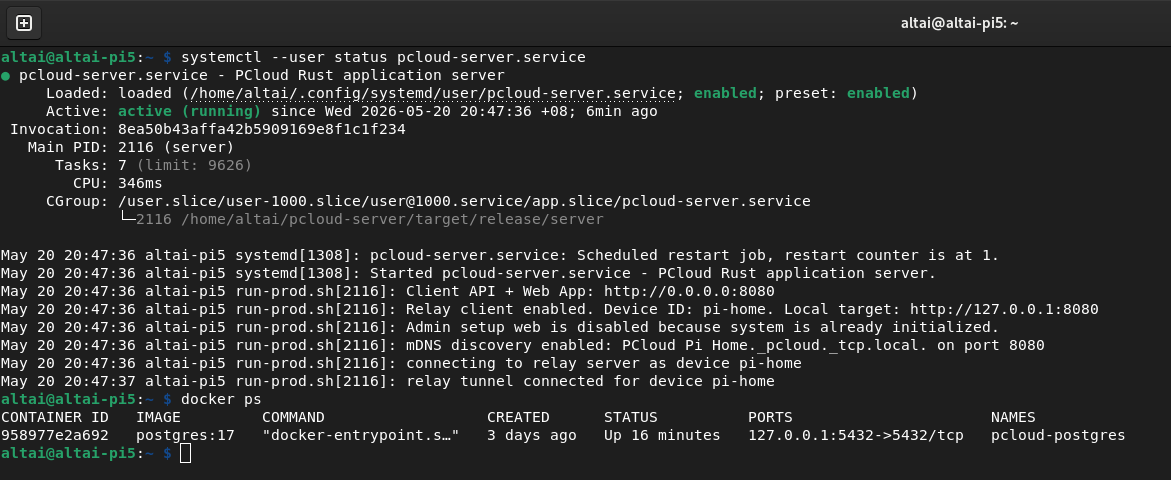
\includegraphics[width=0.95\textwidth]{Figures/chapter4/ssh-pi-main-server-user-service.png}
    \caption{Тухайн Raspberry Pi дээрх ажиллаж буй үндсэн сервер апп ба Postgre бааз}
    \label{fig:ssh-pi-main-server-user-service}
\end{figure}

Тухайн Raspberry pi дээр үндсэн серверийн аппаа ажиллуулсан бол дамжуулагч серверийг Hetzner-ийн төлбөртэй virtual public server-ийг ашигласан. Тухайн авсан сервер дээрээ debian үйлдлийн системийг сонгон ашигласан. Учир нь debian нь маш энгийн бөгөөд серверийн зориулалтаар ашиглагдаад удсан нэр хүндтэй distro юм. Дараах зураг 
\ref{fig:hetzner-admin-console}-т Hetzner-ийн admin console-ийг харуулав.

\begin{figure}[H]
    \centering
    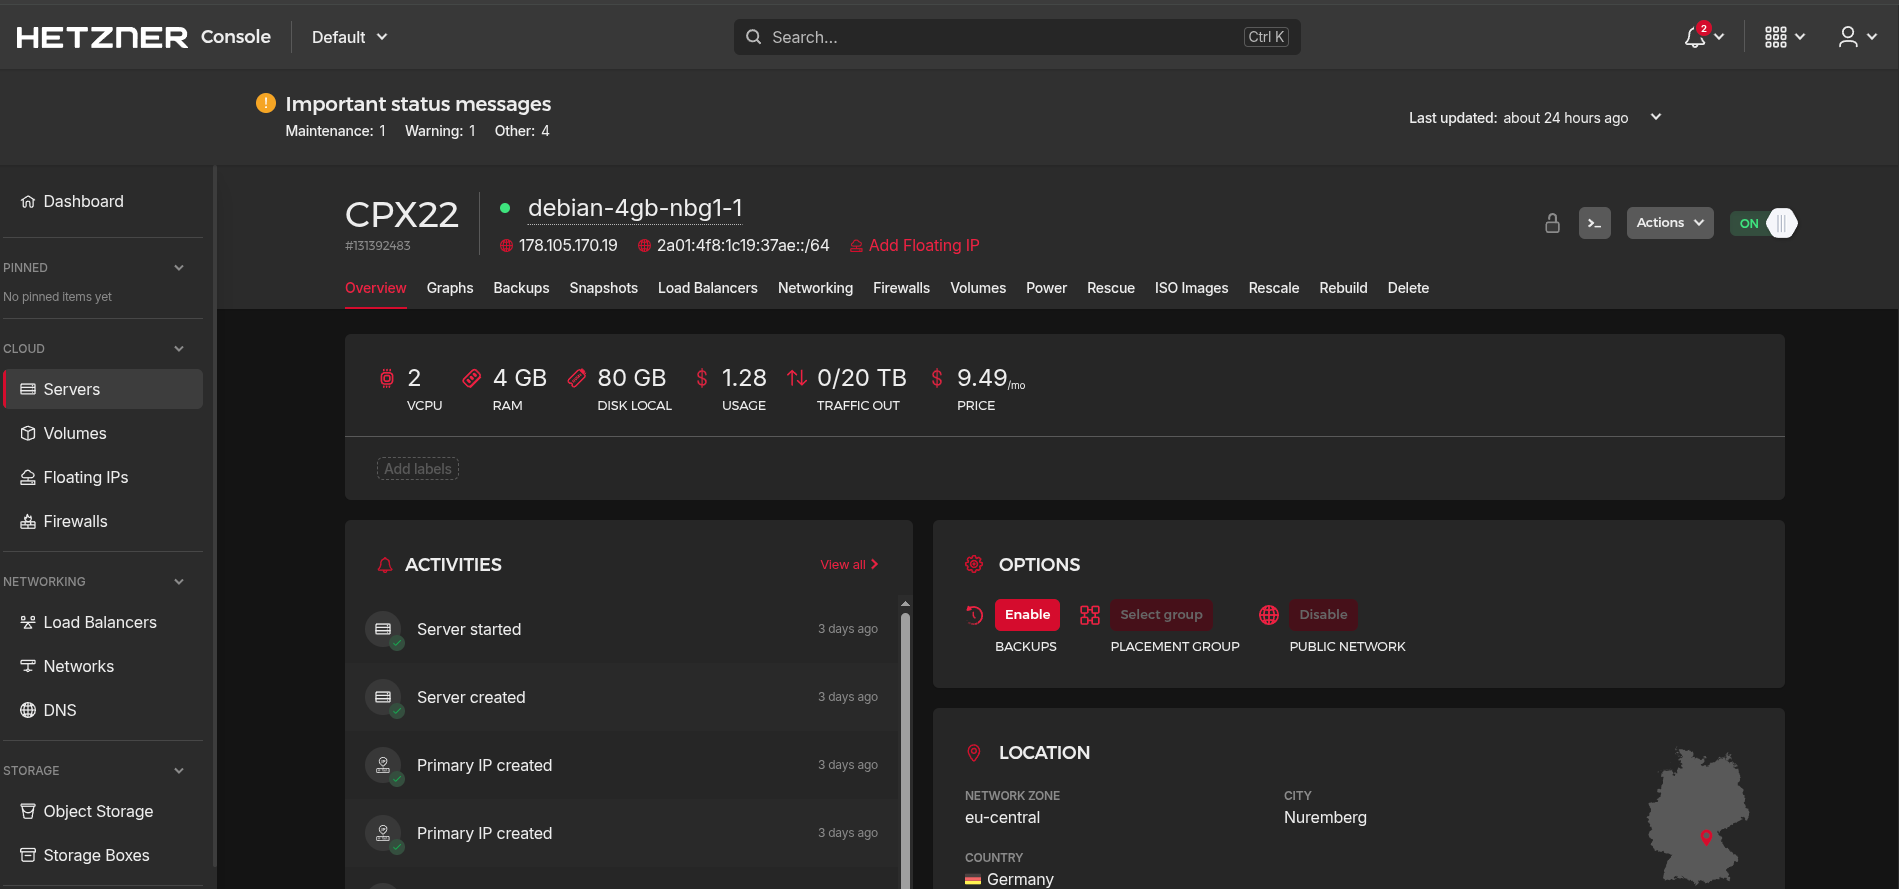
\includegraphics[width=0.95\textwidth]{Figures/chapter4/hetzner-admin-console.png}
    \caption{Hetzner VPS admin console харагдах байдал}
    \label{fig:hetzner-admin-console}
\end{figure}

Дамжуулагч серверийг бүрэн docker compose ашиглан container-жуулсан бөгөөд үндсэн ашиглаж буй 2 container байгааг дараах \ref{fig:hetzner-vps-ssh} зурагт харуулав. Үндсэн relay-1 container нь rust-аас build хийгдсэн executable binary-г ажиллуулдаг. Харин caddy-1 container нь тухайн ажиллах буй relay-server дээр HTTPS холболт хийхэд ашиглаж байгаа. Мөн тухайн VPS-ийн IP болох 178.105.170.19-г cloudflare дээр авсан domain-тойгоо холбож ажиллуулж байгаа.

\begin{figure}[H]
    \centering
    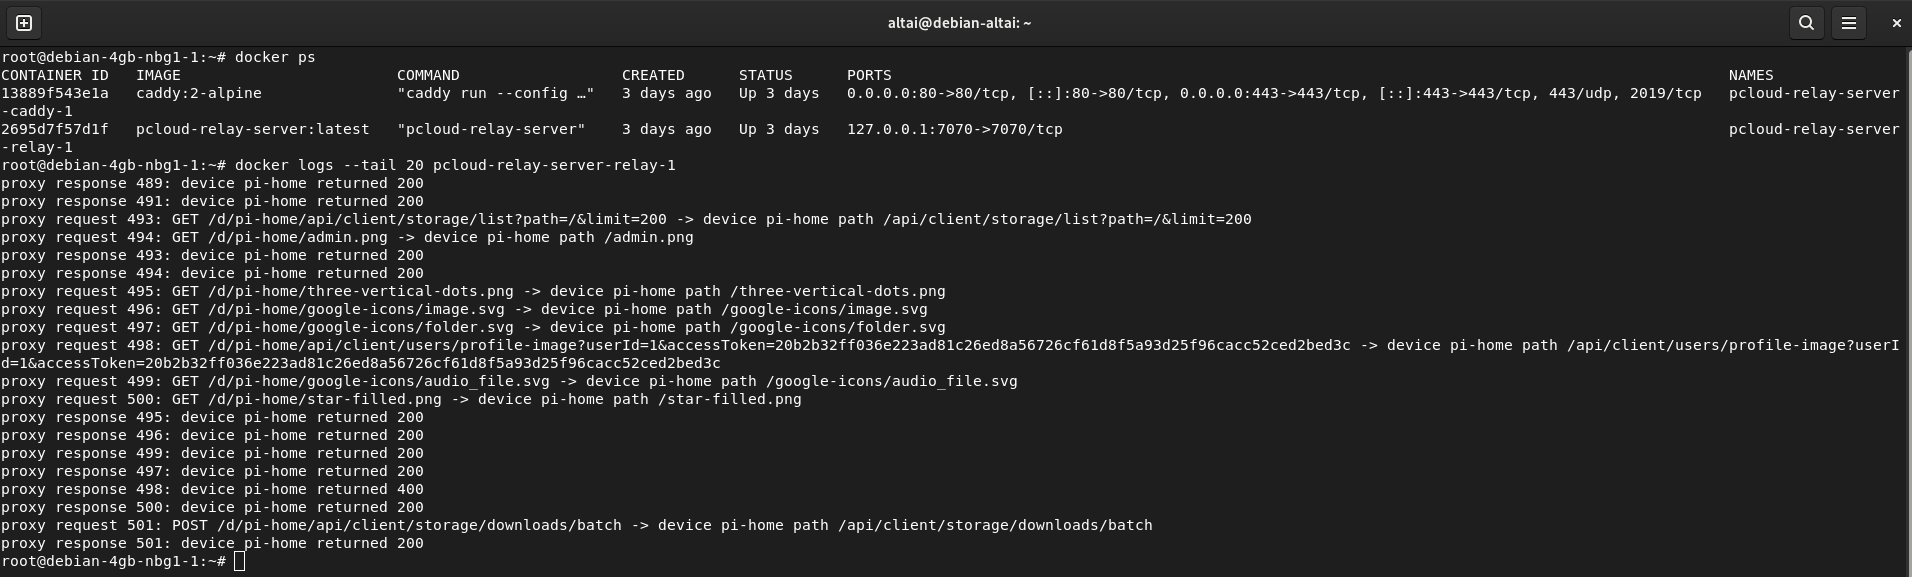
\includegraphics[width=0.95\textwidth]{Figures/chapter4/hetzner-vps-ssh.png}
    \caption{VPS-рүү SSH хандалт хийж байгаа байдал}
    \label{fig:hetzner-vps-ssh}
\end{figure}

\section{Системийн холболтын ажиллагаа}

\section{Хөгжүүлсэн системийн интерфейс}

\paragraph{}
Зураг~\ref{fig:dev-admin-init}-т системийг анх ажиллуулах үед гарч ирэх анхны тохиргооны дэлгэцийг харуулав. Энэ дэлгэцэд хэрэглэгч админ бүртгэлийн нэр болон нууц үг, мөн файлуудыг хадгалах серверийн замыг тохируулна. Энэхүү анхны тохиргоог амжилттай дуусгасны дараа систем хэвийн ажиллах бэлэн болно.

\begin{figure}[H]
    \centering
    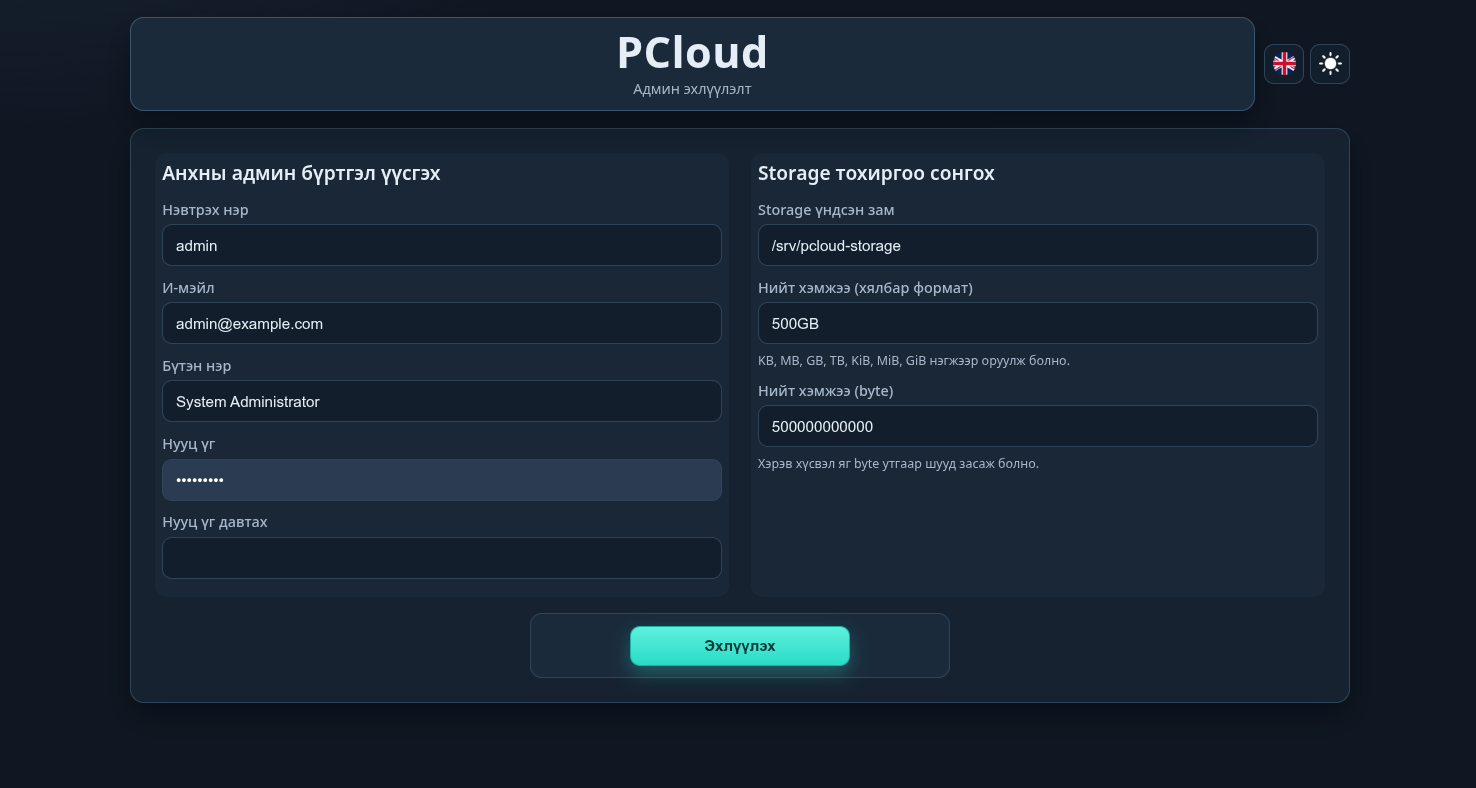
\includegraphics[width=0.70\textwidth]{Figures/chapter3/developed-interfaces/admin-initialize.png}
    \caption{Анхны тохиргооны дэлгэц}
    \label{fig:dev-admin-init}
\end{figure}


\paragraph{}
Зураг~\ref{fig:dev-login-web}-д веб клиентийн нэвтрэх дэлгэцийг харуулав. Серверийн хаяг, хэрэглэгчийн нэр болон нууц үг оруулах талбарууд байх бөгөөд self-hosted системд өөр өөр серверт холбогдох боломжийг олгодог.

\begin{figure}[H]
    \centering
    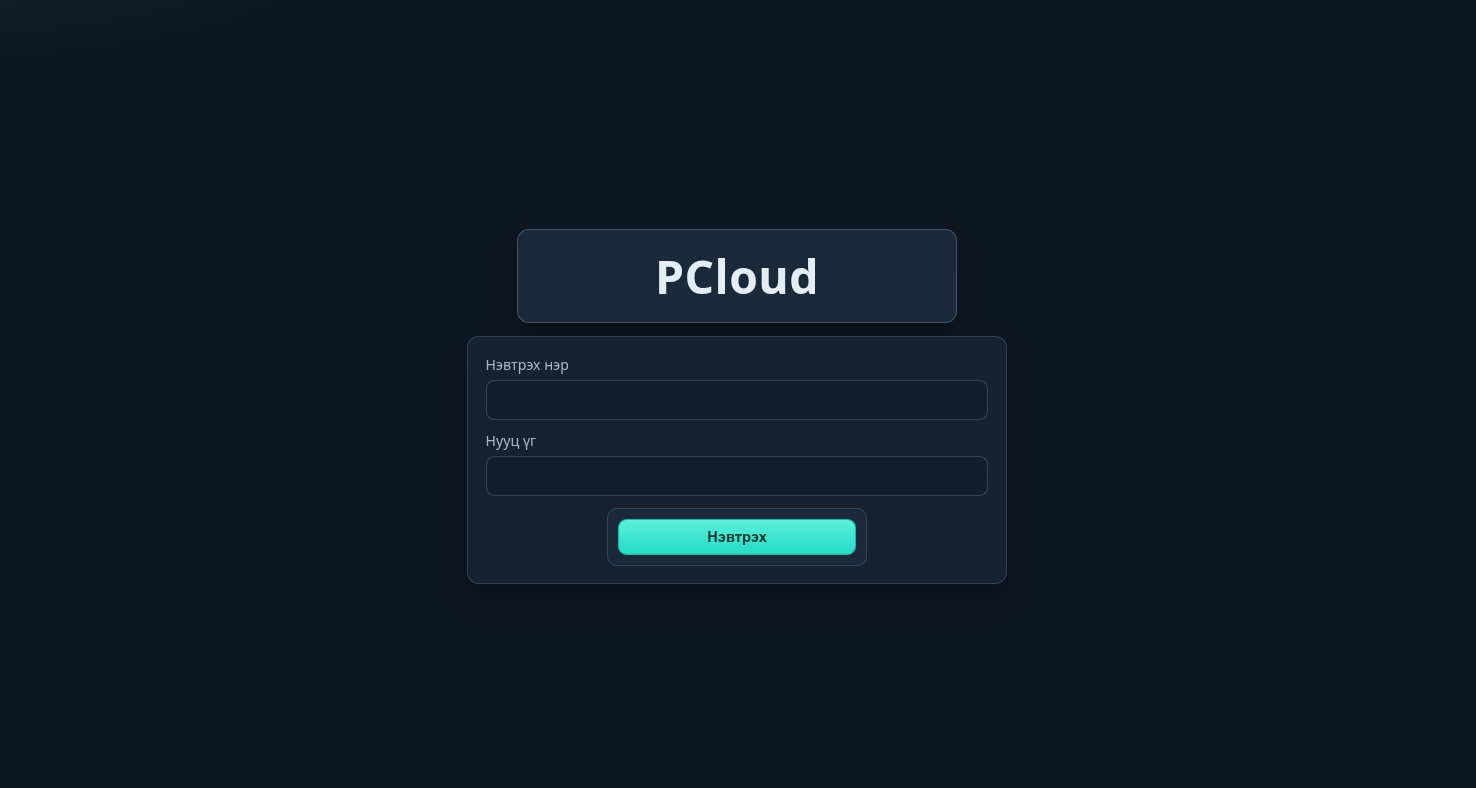
\includegraphics[width=0.85\textwidth]{Figures/chapter3/developed-interfaces/login.png}
    \caption{Веб нэвтрэх дэлгэц}
    \label{fig:dev-login-web}
\end{figure}

\paragraph{}
Зураг~\ref{fig:dev-login-mobile}-д мобайл клиентийн нэвтрэх дэлгэцийг харуулав. Веб хувилбарттай адил талбаруудыг агуулах бөгөөд мобайл дэлгэцийн хэмжээнд тохирсон компакт байршилтай.

\begin{figure}[H]
    \centering
    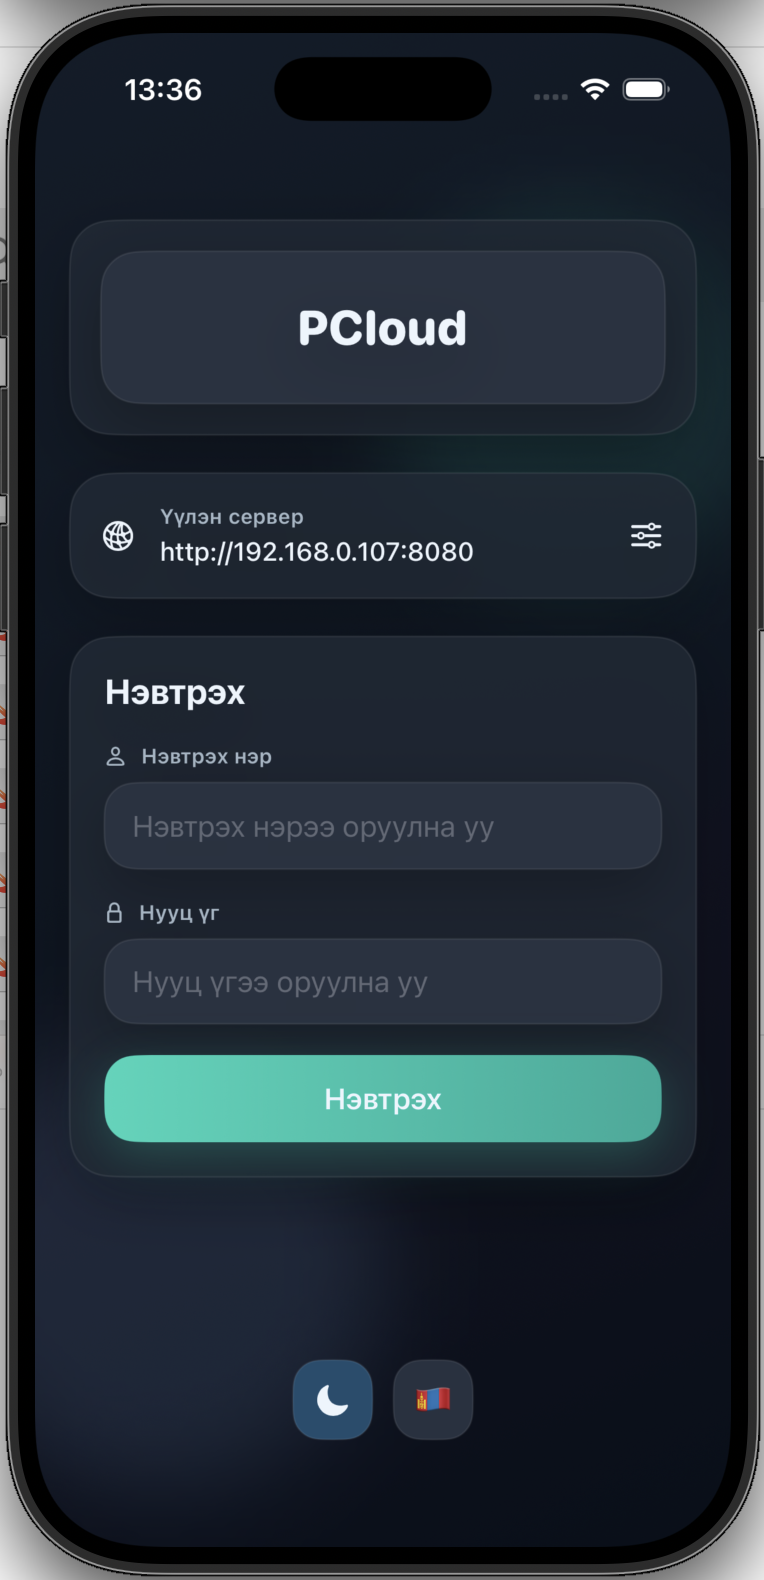
\includegraphics[width=0.35\textwidth]{Figures/chapter3/developed-interfaces/mobile-login-page.png}
    \caption{Мобайл нэвтрэх дэлгэц}
    \label{fig:dev-login-mobile}
\end{figure}

\paragraph{}
Зураг~\ref{fig:dev-dark-home-web}-д хэрэглэгчийн нүүр хуудасны харанхуй горимын веб хувилбарыг харуулав. Файл болон хавтасны бүтэц жагсаалт хэлбэрээр харагдах бөгөөд upload, download, нэр өөрчлөх, устгах зэрэг үндсэн үйлдлүүдийг хийх боломжтой.

\begin{figure}[H]
    \centering
    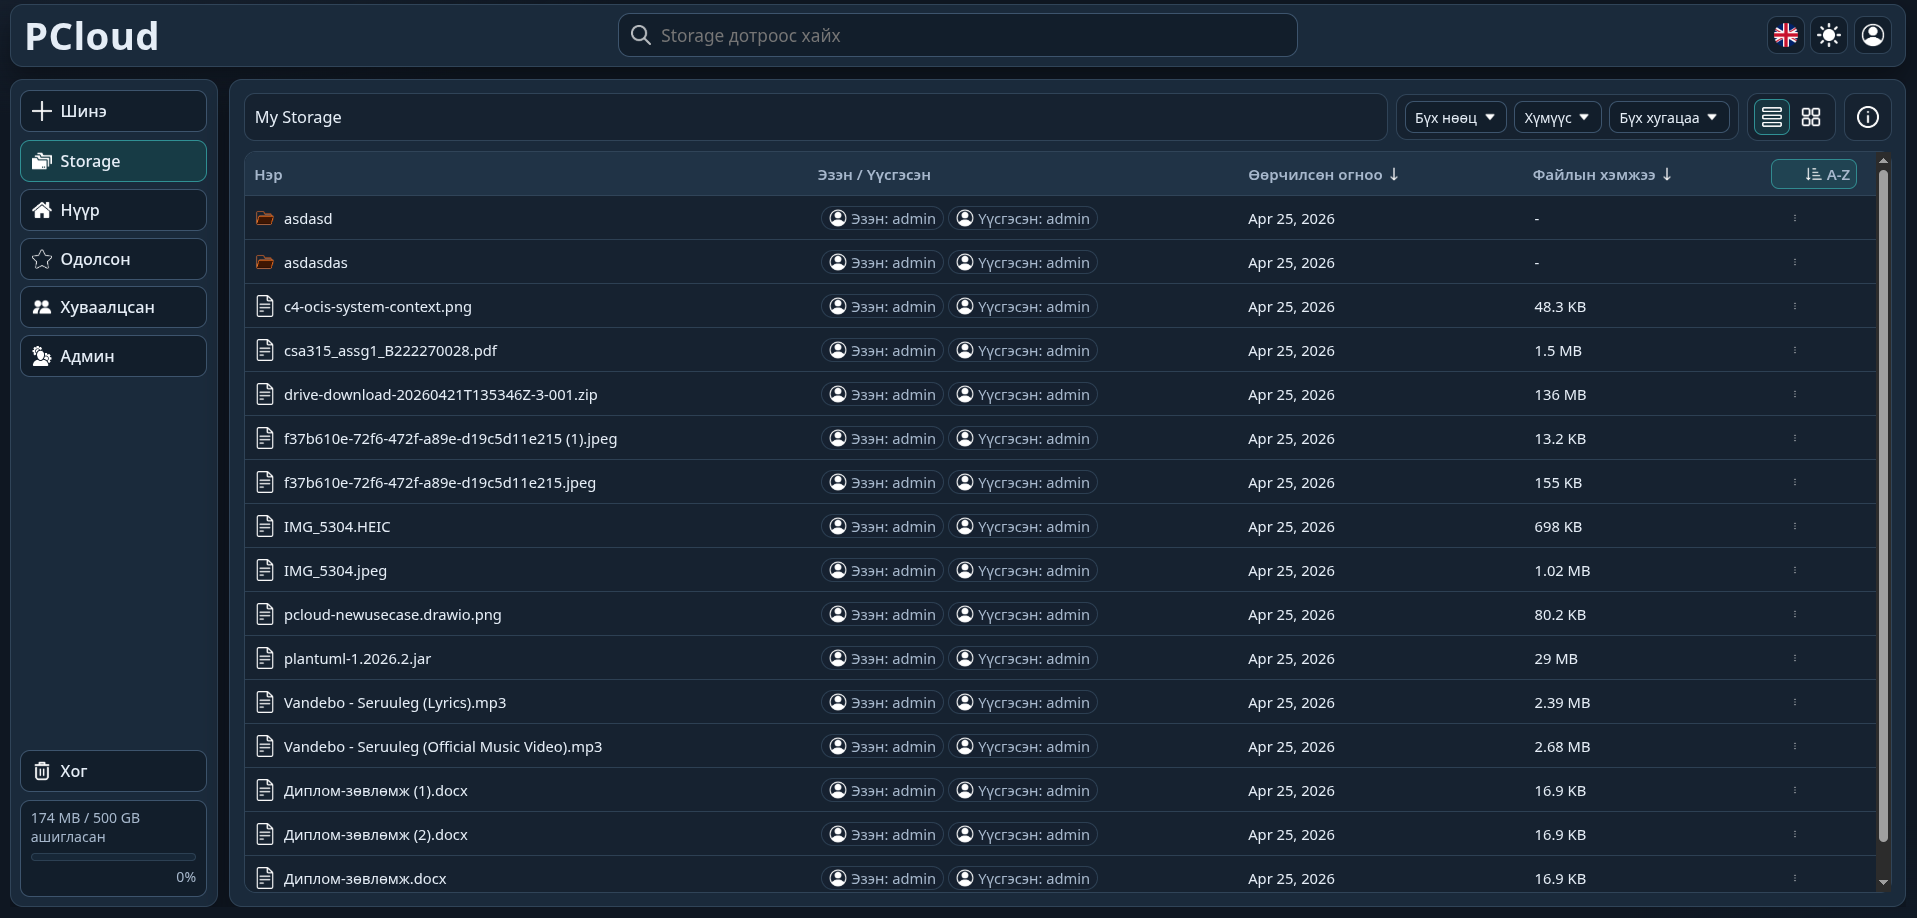
\includegraphics[width=0.85\textwidth]{Figures/chapter3/developed-interfaces/home-page-dark-mode.png}
    \caption{Веб нүүр хуудас -- харанхуй горим}
    \label{fig:dev-dark-home-web}
\end{figure}

\paragraph{}
Зураг~\ref{fig:dev-dark-home-mobile}-д мобайл клиентийн харанхуй горимын нүүр хуудасыг харуулав. Веб хувилбарын нэгэн адил үндсэн файл удирдлагын үйлдлүүд мобайл дэлгэцийн хэмжээнд тохирсон хэлбэрт харагдана.

\begin{figure}[H]
    \centering
    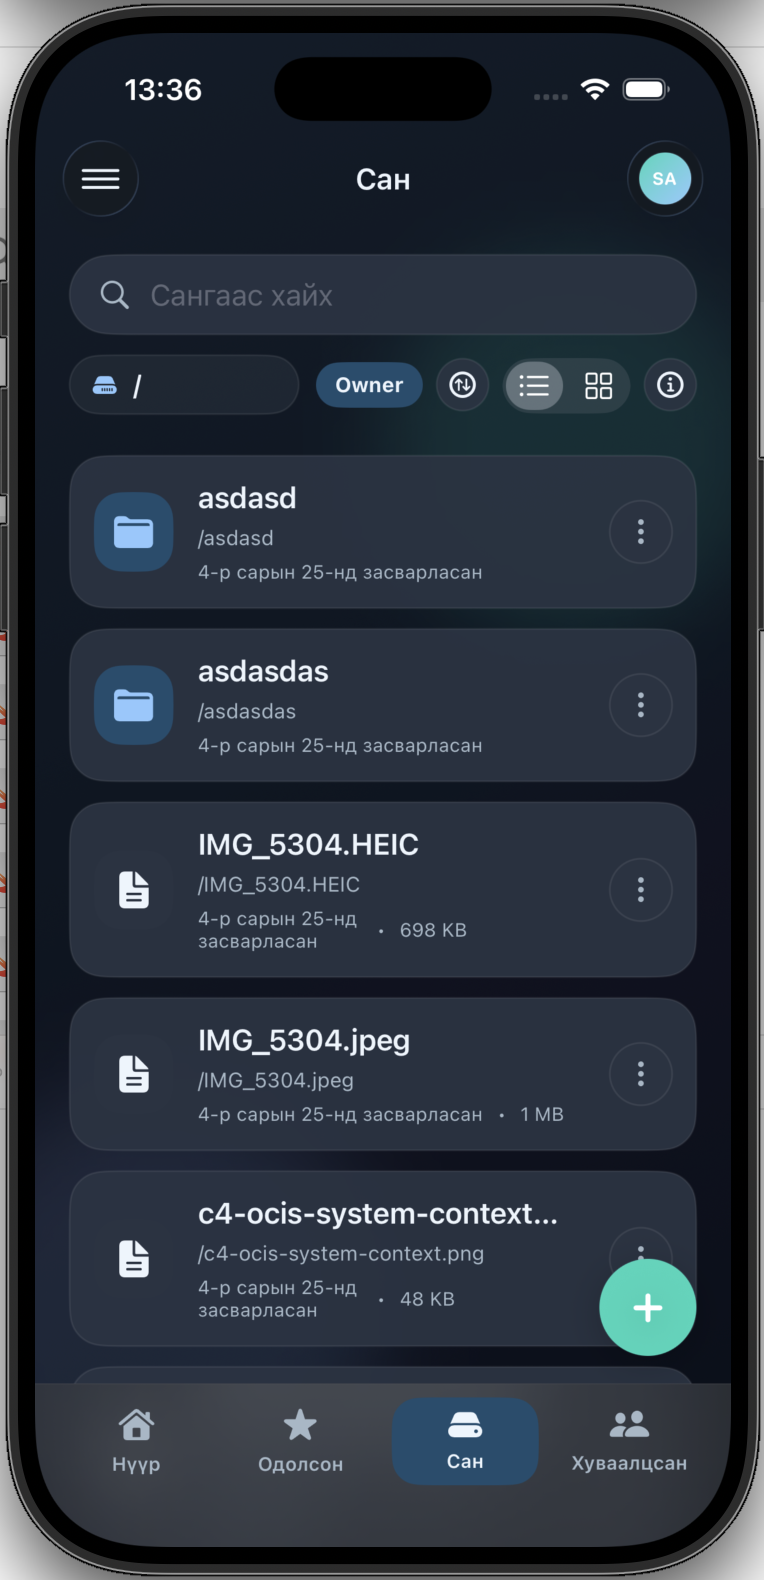
\includegraphics[width=0.35\textwidth]{Figures/chapter3/developed-interfaces/mobile-home-page-dark-mode.png}
    \caption{Мобайл нүүр хуудас -- харанхуй горим}
    \label{fig:dev-dark-home-mobile}
\end{figure}

\section{Туршилтын арга зүй}

\section{Туршилтын үр дүн}

\chapterconclusiontitle{Бүлгийн дүгнэлт}
\paragraph{}
Энэ бүлэгт гуравдугаар бүлэгт тодорхойлсон зохиомжийг бодит систем болгон хэрэгжүүлсэн байдал, хэрэглэгчийн интерфейсийн бодит хувилбарууд, нэвтрүүлэлтийн орчин болон туршилтын үр дүнг тайлбарлалаа. Үндсэн серверийг хэрэглэгчийн өөрийн төхөөрөмж дээр ажиллуулж, веб болон мобайл клиентээр дамжуулан файл удирдах үндсэн урсгалуудыг шалгаснаар системийн зорилго болох self-hosted хувийн үүлэн хадгалалтын үндсэн боломжууд хэрэгжих боломжтойг харууллаа.
